\documentclass{article}

% Language setting
\usepackage[english]{babel}

% Set page size and margins
\usepackage[a4paper,top=2cm,bottom=2cm,left=3cm,right=3cm,
	marginparwidth=1.75cm]{geometry}

% Useful packages
\usepackage{amsmath}
\usepackage{graphicx}
\usepackage[colorlinks=true, allcolors=blue]{hyperref}

\usepackage{footmisc}

\usepackage{tikz}
\usetikzlibrary{shapes,arrows,positioning,fit,backgrounds}

\title{
	Evaluating the Vertical and Horizontal Read and Write Scalability of 
	MobilityDB and CrateDB
	\\[1ex] \large Bachelor's Thesis Exposé}
\author{Eryk Karol Kściuczyk}
\date{} % This removes the date

\begin{document}
\maketitle

% Context
Spatio-temporal databases are increasing in popularity due to increased
production of such data by numerous IoT devices.
As the need for such databases increases, developers try to reach for 
familiar and open-source solutions.
MobilityDB, built on top of the spatial extension PostGIS, extends PostgreSQL's 
capabilities regarding spatio-temporal aspects.
Previous research has shown that MobilityDB can also scale horizontally using
another extension, Citus.
As a comparison, CrateDB is a natively distributable SQL database designed for
scalability and high performance.

% Problem Statement
While the runtimes of specific queries of BerlinMOD benchmark have been 
evaluated on 4 and 28 node clusters of MobilityDB,
its horizontal and vertical scalability still remains underexplored.
Previous research mostly focuses on designing queries for single node systems,
and often does not compare systems between one another. 
Another option, CrateDB, also has not been fully evaluated for its usability 
in spatiotemporal use cases.
Moreover, benchmarking with a wider range of cluster sizes is necessary to 
establish the scalability pattern.
Additionally, a comparison between MobilityDB+Citus and CrateDB in terms of
horizontal scalability has not been conducted, which could provide valuable
insights into their respective strengths and weaknesses.

% Solution Approach
In this thesis we implement a spatiotemporal benchmark that evaluates the
scalability of relational databases both horizontally and vertically.
We build a data generation and benchmarking tool to stress the respective 
systems (MobilityDB and CrateDB). The benchmark setup can be seen on figure 
\ref{fig:bench_setup}.

% Hard implementation details
We will compare the performance of the distributed MobilityDB and 
CrateDB on different hardware configurations using Google Cloud Platform.
Additionally, we will evaluate several scenarios, including vertically scaling 
a single node and scaling out by distributing both solutions across several
instances. 
We use our benchmark results to evaluate the systems for their scalability
and also compare their performance against each other.

\begin{figure}[ht]
	\centering
	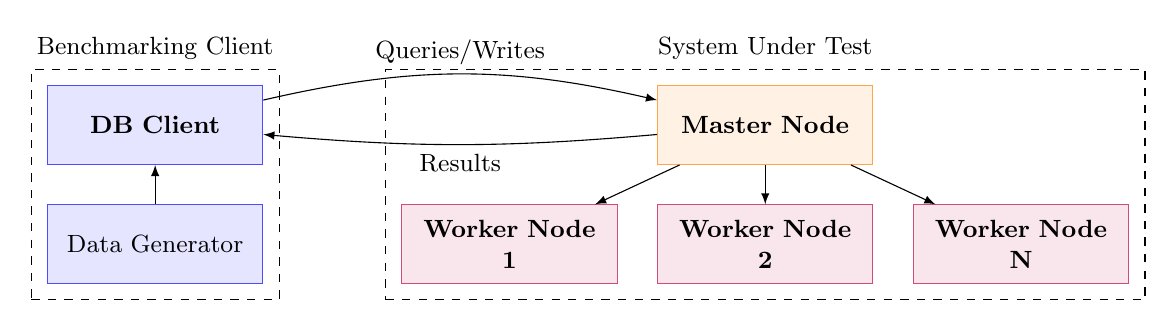
\begin{tikzpicture}[
	font=\small,
		node distance=0.5cm,
		box/.style={
			rectangle,
			draw,
			text width=2.5cm,
			minimum height=1cm,
			align=center
		},
		client/.style={
			box,
			fill=blue!10,
			draw=blue!70
		},
		coordinator/.style={
			box,
			fill=orange!10,
			draw=orange!70,
		},
		worker/.style={
			box,
			fill=purple!10,
			draw=purple!70
		},
		group/.style={
			rectangle,
			draw,
			dashed,
			inner sep=0.2cm
		},
		arrow/.style={
			->,
			>=latex
		}
	]
	% Client components
	\node[client] (db_client) {\textbf{DB Client}};
	\node[client, below=of db_client] (datagen) {Data Generator};
	% Client connections
	\draw[arrow] (datagen) -- (db_client);
	% Coordinator node
	\node[coordinator, right=5cm of db_client] (cn) {
		 \textbf{Master Node}};
	% Worker nodes
	\node[worker, below=of cn] (w2) {
		\textbf{Worker Node \\ 2}};
	\node[worker, left=of w2] (w1) {
		\textbf{Worker Node \\ 1}};
	\node[worker, right=of w2] (w3) {
		\textbf{Worker Node \\ N}};
	% Connections of coordinator to workers
	\draw[arrow] (cn) -- (w1);
	\draw[arrow] (cn) -- (w2);
	\draw[arrow] (cn) -- (w3);
	% Client to SUT connections
	\draw[arrow] (db_client) to[bend left=13] node[above] {Queries/Writes} (cn);
	\draw[arrow] (cn) to[bend left=5] node[below] {Results} (db_client);
	
	% Group boxes
	\begin{pgfonlayer}{background}
		% Benchmarking client
		\node[group, fit=(db_client) (datagen)] (client) {};
		\node[above] at (client.north) {Benchmarking Client};

		% System Under test
		\node[group, fit=(cn) (w1) (w2) (w3)] (sut) {};
		\node[above] at (sut.north) {System Under Test};
	\end{pgfonlayer}
	\end{tikzpicture}
	\caption{
 	Benchmarking client will write generated spatiotemporal data and execute
	the workload against System Under Test (MobilityDB/CrateDB cluster).
	The cluster consists of a single master node and multiple worker nodes
	}
	\label{fig:bench_setup}
\end{figure}

% Analysis/ Evaluation
We measure metrics such as query latency and write throughput using confidence
intervals, while also visualizing the distribution using Empirical Cumulative
Distribution Function (ECDF) plots, to reveal performance patterns and tail 
latencies.
We repeat each experiment multiple times to ensure the validity of our results.
\end{document}
